\documentclass[11pt]{article}
\usepackage[utf8]{inputenc}
\usepackage{amsmath,amssymb}
\usepackage{graphicx}
\usepackage{hyperref}
\usepackage{geometry}
\geometry{margin=1in}

% --- TikZ and PGFPlots for waveforms (Optional) ---
\usepackage{tikz}
\usepackage{pgfplots}
\pgfplotsset{compat=1.18}  % Adjust if necessary

\title{A Hierarchical Framework of Emotion Using EAR and Good/Bad Valued Logic}
\author{Brian Searls\\\href{https://github.com/briansrls}{https://github.com/briansrls}}
\date{\today}

\begin{document}

\maketitle

\begin{abstract}
This paper outlines a hierarchical model of emotions based on an \textbf{Event-Appraisal-Response (EAR)} framework and Good/Bad valued logic. Emotions are categorized at three levels (L0--L2). At the foundation (L0) are fundamental positive (\textit{Good}) and negative (\textit{Bad}) affective signals. Building on these, early discrete emotions (\textit{Interest, Disgust}) appear at L1. Finally, more complex emotions (\textit{Fear, Anger, Sadness, Surprise}) emerge at L2 as combinations of lower-level states or further interactions of Good and Bad signals. We present an adjacency matrix summarizing how each node influences the others, and then show how time-varying functions \(G(t)\) and \(B(t)\) capture the temporal dynamics of emotional responses. Example waveforms for \textit{Surprise} and \textit{Fear} illustrate these dynamics in action. Future work will consider extending this framework to higher-level emotions (L3+).
\end{abstract}

\tableofcontents

\section{Introduction}
Emotions are central to cognition, communication, and behavior. Numerous psychological and computational models have explored their structure, function, and development. In this framework, we use \textbf{Event-Appraisal-Response (EAR)} as a conceptual lens: an \textit{event} occurs, the system \textit{appraises} it in terms of valence (good/bad), and produces a \textit{response} in the form of an emotional state. Alongside EAR, we incorporate a Good/Bad valued logic that posits two core affective signals—\textit{Good} and \textit{Bad}—as the foundation on which more nuanced emotions are built.

Sections \ref{sec:hierarchy} and \ref{sec:matrix} detail a three-level emotional hierarchy (L0--L2) and summarize the key connections among the nodes via an adjacency matrix. Section \ref{sec:dynamics} introduces the functions \(G(t)\) and \(B(t)\), which evolve over time to capture shifting positive and negative valence. Section \ref{sec:waveform-examples} provides waveform examples for \textit{Surprise} and \textit{Fear} using TikZ and PGFPlots. Finally, Section \ref{sec:conclusion} discusses future directions, including higher-level (L3+) emotions.

\section{Three Levels of Emotional Emergence}
\label{sec:hierarchy}
This model posits a three-level emotional structure:

\subsection{L0: Fundamental Good/Bad States}
\begin{itemize}
    \item \textbf{Good (positive valence)}: A fundamental feeling of pleasure, comfort, or satisfaction.
    \item \textbf{Bad (negative valence)}: A fundamental feeling of discomfort, pain, or distress.
\end{itemize}

\subsection{L1: Early Emotions (Interest, Disgust)}
\begin{itemize}
    \item \textbf{Interest}: A positive, exploratory state triggered by novelty or anticipated opportunity (primarily Good with a slight uncertainty component).
    \item \textbf{Disgust}: An aversive response to something judged unpleasant, harmful, or offensive (primarily Bad).
\end{itemize}

\subsection{L2: Complex Emotions (Fear, Anger, Sadness, Surprise)}
\begin{itemize}
    \item \textbf{Fear}: Triggered by a perceived threat, often combining a strong Bad signal with alarm or vigilance.
    \item \textbf{Anger}: Arises from blocked goals or perceived injustice, reflecting both Good (the desired outcome) and Bad (the obstacle or violation).
    \item \textbf{Sadness}: A sustained negative state tied to the loss of something previously Good or an enduring adversity.
    \item \textbf{Surprise}: A brief, intense reaction to the unexpected, potentially involving both startle (negative) and curiosity (positive).
\end{itemize}

\section{Adjacency Matrix of Connections}
\label{sec:matrix}
Table~\ref{tab:adjacency-matrix} summarizes how each node (L0--L2) influences every other node in this framework. We use the following abbreviations:

\begin{itemize}
    \item “--”: No self-connection.
    \item “-”: No or negligible influence.
    \item “Strong”, “Partial”, “Brief”, “Sustained”: Qualitative descriptors of influence strength.
\end{itemize}

\begin{table}[htbp]
\centering
\renewcommand{\arraystretch}{1.15}
\resizebox{\textwidth}{!}{%
\begin{tabular}{l|cccccccc}
\hline
 & \textbf{Good(L0)} & \textbf{Bad(L0)} & \textbf{Interest(L1)} & \textbf{Disgust(L1)} & \textbf{Fear(L2)} & \textbf{Anger(L2)} & \textbf{Sadness(L2)} & \textbf{Surprise(L2)} \\
\hline
\textbf{Good(L0)}      & -- & - & Strong & Weak & - & Partial & Sustained & Partial \\
\textbf{Bad(L0)}       & - & -- & Weak & Strong & Strong & Partial & Strong & Partial \\
\textbf{Interest(L1)}  & - & - & -- & - & Strong & Partial & - & Brief \\
\textbf{Disgust(L1)}   & - & - & - & -- & Partial & Strong & - & Brief \\
\hline
\end{tabular}
}
\caption{Adjacency matrix for L0--L2 nodes. Each cell indicates the qualitative nature of influence. The diagonal is ``--'' to denote no self-connections.}
\label{tab:adjacency-matrix}
\end{table}

\section{Temporal Dynamics of Good/Bad Signals}
\label{sec:dynamics}
In addition to structural connections, we view each emotion as a pattern in two time-varying signals:
\[
G(t) \quad\text{(Good component)}, 
\quad 
B(t) \quad\text{(Bad component)},
\]
where events trigger changes in \(G(t)\) and/or \(B(t)\). This aligns with EAR by positing that once an event is appraised, the system shifts these valences, ultimately producing a response (emotion).

\subsection{Illustrative Formalism}
A common approach is exponential decay:
\[
G(t) \;=\; \sum_{i} \Delta G_i \, e^{-\alpha (t - t_i)}\, H(t - t_i), 
\quad
B(t) \;=\; \sum_{j} \Delta B_j \, e^{-\beta (t - s_j)}\, H(t - s_j),
\]
where each event contributes a “pulse” of Good or Bad with amplitude \(\Delta G_i\) or \(\Delta B_j\), decaying at rates \(\alpha\) or \(\beta\). The Heaviside step function \(H(\cdot)\) ensures the contribution starts only after the event time.

\section{Waveform Examples: Surprise and Fear}
\label{sec:waveform-examples}
We now illustrate two distinct emotional profiles under the EAR framework: \textbf{Surprise}, which often involves both a positive and negative spike, and \textbf{Fear}, featuring predominantly negative activation.

\subsection{Surprise}
An event at \(t=1\) triggers both a positive spike (\(G(t)\)) and a negative spike (\(B(t)\)), interpreted as startle plus curiosity. Figure~\ref{fig:surprise-waveform} shows a hypothetical plot.

\begin{figure}[htbp]
\centering
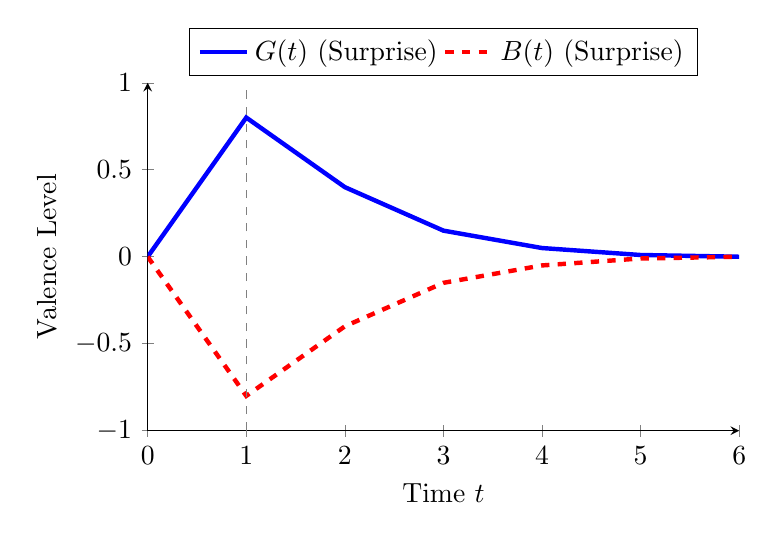
\begin{tikzpicture}
\begin{axis}[
    width=0.75\textwidth,
    height=6cm,
    xmin=0, xmax=6,
    ymin=-1, ymax=1,
    axis lines=left,
    xlabel={Time $t$},
    ylabel={Valence Level},
    ytick={-1, -0.5, 0, 0.5, 1},
    legend style={at={(0.5,1.02)},anchor=south,legend columns=2}
]
% G(t) for Surprise
\addplot[blue, ultra thick] coordinates {
    (0, 0)
    (1, 0.8)
    (2, 0.4)
    (3, 0.15)
    (4, 0.05)
    (5, 0.01)
    (6, 0)
};
\addlegendentry{$G(t)$ (Surprise)}

% B(t) for Surprise
\addplot[red, ultra thick, dashed] coordinates {
    (0, 0)
    (1, -0.8)
    (2, -0.4)
    (3, -0.15)
    (4, -0.05)
    (5, -0.01)
    (6, 0)
};
\addlegendentry{$B(t)$ (Surprise)}

% Event line
\draw[dashed,gray] (axis cs:1,-1) -- (axis cs:1,1)
  node[above,pos=1,black]{Event at $t=1$};

\end{axis}
\end{tikzpicture}
\caption{Hypothetical Surprise response showing simultaneous spikes in $G(t)$ (positive) and $B(t)$ (negative). Both signals decay over time.}
\label{fig:surprise-waveform}
\end{figure}

\subsection{Fear}
In contrast, a Fear response might produce a sharp negative spike while \(G(t)\) remains near zero. Figure~\ref{fig:fear-waveform} shows an event at \(t=2\) driving \(B(t)\) strongly negative, reflecting a threat appraisal.

\begin{figure}[htbp]
\centering
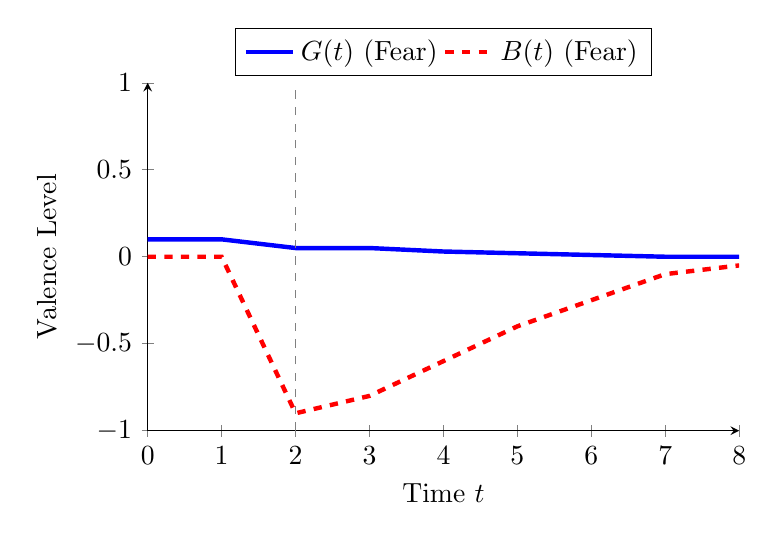
\begin{tikzpicture}
\begin{axis}[
    width=0.75\textwidth,
    height=6cm,
    xmin=0, xmax=8,
    ymin=-1, ymax=1,
    axis lines=left,
    xlabel={Time $t$},
    ylabel={Valence Level},
    ytick={-1, -0.5, 0, 0.5, 1},
    legend style={at={(0.5,1.02)},anchor=south,legend columns=2}
]
% G(t) for Fear
\addplot[blue, ultra thick] coordinates {
    (0, 0.1)
    (1, 0.1)
    (2, 0.05)
    (3, 0.05)
    (4, 0.03)
    (5, 0.02)
    (6, 0.01)
    (7, 0)
    (8, 0)
};
\addlegendentry{$G(t)$ (Fear)}

% B(t) for Fear
\addplot[red, ultra thick, dashed] coordinates {
    (0, 0)
    (1, 0)
    (2, -0.9)
    (3, -0.8)
    (4, -0.6)
    (5, -0.4)
    (6, -0.25)
    (7, -0.1)
    (8, -0.05)
};
\addlegendentry{$B(t)$ (Fear)}

% Dashed event line
\draw[dashed,gray] (axis cs:2,-1) -- (axis cs:2,1)
  node[above,pos=1,black]{Event at $t=2$};

\end{axis}
\end{tikzpicture}
\caption{Hypothetical Fear response. $B(t)$ spikes downward at $t=2$ while $G(t)$ remains minimal, indicating a primarily negative affective state.}
\label{fig:fear-waveform}
\end{figure}

\section{Conclusion and Outlook}
\label{sec:conclusion}
This paper introduced a hierarchical model of emotions grounded in \textbf{Event-Appraisal-Response (EAR)} principles and a Good/Bad valued logic. The framework encompasses three levels (L0--L2), starting with fundamental valences (\textit{Good, Bad}), proceeding to early discrete emotions (\textit{Interest, Disgust}), and culminating in more complex secondary emotions (\textit{Fear, Anger, Sadness, Surprise}). An adjacency matrix was provided to outline the relationships among these nodes, while time-dependent valence signals \((G(t), B(t))\) illustrated how emotional states unfold under various conditions.

In future work, this approach could be extended to L3 and beyond, capturing self-conscious emotions such as guilt, pride, or shame, which incorporate more elaborate cognitive appraisals yet still rely on the fundamental Good/Bad axis. Potential applications range from developmental psychology to affective computing and artificial intelligence, offering a structured, valence-based way to simulate or interpret emotional processes under the EAR model.

\end{document}
